\documentclass[a4paper]{article}
\usepackage[italian]{babel}
\usepackage[left=2cm, right=2cm, bottom=2cm, top=2cm]{geometry}
\usepackage{csvsimple}
\usepackage[utf8]{inputenc}
\usepackage{float}
\usepackage{pdfpages}
\usepackage[scaled]{helvet}
\renewcommand\familydefault{\sfdefault} 
\usepackage{pgfplots}
\usepackage{pdflscape}
%opening
\title{Relazione laboratorio Algoritmi Avanzati}
\author{Magarotto Francesco\\Muraro Enrico\\Piva Giulio}

\begin{document}
\begin{titlepage}
  \vspace*{5cm}
  \begin{center}
    \Large\bfseries
    Relazione di laboratorio
  \end{center}
  \begin{center}
    \large
    Corso di Algoritmi Avanzati\\
    Laurea Magistrale in Informatica\\A.A. 2019-2020
  \end{center}
  \vspace{4cm plus 1fill}
  \begin{flushleft}
    \large
    Magarotto Francesco - 1236594\\Muraro Enrico - 1238899 \\Piva Giulio - 1242455
  \end{flushleft}
\end{titlepage}
\newpage

\section{Introduzione}

è valutare le prestazioni dell'algoritmo di Karger per il problema del minimum cut rispetto a quattro parametri:
\begin{itemize}
\item Il tempo impiegato dalla procedura di Full Contraction
\item Il tempo impiegato dall'algoritmo completo per ripetere la contrazione un numero sufficientemente alto di volte
\item Il discovery time, ossia il momento in cui l'algoritmo trova per la prima volta il taglio di costo mimimo
\item L'errore nella soluzione trovata rispetto al risultato ottimo
\end{itemize}
Il linguaggio di programmazione scelto dal nostro gruppo è Java.

\subsection{Esecuzione del programma}
Gli algoritmi sono stati sviluppati come progetto Maven. All'interno della cartella \'e presente la versione portable di Maven, pertanto non è necessario averlo installato. \'E
richiesto almeno il JDK 11 installato nel sistema.
Per eseguire i tre algoritmi utilizzare i seguenti comandi:\\
Linux:\\
\indent \texttt{./mvnw install}\\
\indent \texttt{./mvnw exec:java}\\
Windows:\\
\indent \texttt{mvnw.cmd install}\\
\indent \texttt{mvnw.cmd exec:java}

L'esecuzione del main genera automaticamente dei file csv nella directory del progetto contenenti i tempi registrati. L'algoritmo di Karger viene interrotto dopo 60 secondi.
\subsection{Strutture dati utilizzate}

Per rappresentare il grafo abbiamo utilizzato una matrice di adiacenza visto che i sono grafi completi e la matrice viene quindi riempita senza sprechi di memoria.

Nell'algoritmo 2 Approssimato abbiamo fatto uso di un HashMap per registrare la visita in preordine del grafo.

La classe Heap è una nostra implementazione di MinHeap. L'albero binario è rappresentato da un array di interi, i valori all'interno dell'array corrispondono ai nodi presenti nel grafo. Il confronto tra i nodi per determinare il più piccolo è effettuato tramite un Comparator passato alla creazione dello Heap, questo per avere un'implementazione di Heap indipendente dal modo in cui viene utilizzato da uno specifico algoritmo.
\subsection{Lettura di un grafo da file}
Per caricare un grafo in memoria, abbiamo implementato una classe GraphReader, che si occupa della lettura del file tramite la libreria \textit{nio} di Java. Inoltre effettua le conversioni di distanza necessarie sia per i file di tipo GEO che EUC\_2D e ritorna direttamente la matrice di adiacenza del grafo.


\subsection{Implementazione di Held-Karp}

L'algoritmo di Held-Karp necessita di due strutture di supporto, una per salvare le distanze minime già calcolate e una per ricordare il nodo precedente in modo da poter ricostruire il percoso trovato. Visto che entrambi sono identificati da due valori (v,S) dove 'v' è un nodo e 'S' un insieme di nodi abbiamo deciso di implementare entrambe con ArrayList di HashMap. Ogni posizione dell'ArrayList corrisponde a un nodo e contiene una mappa che ha come chiave un Set di nodi. In questo modo con due accessi costanti possiamo trovare il valore desiderato.

Il timeout di Held-Karp è controllato da un flag booleano, quando viene impostato il valore del flag a 'true' il ciclo che cerca il minimo viene interrotto e l'algoritmo ritorna la soluzione migliore trovata fino a quel momento.

Quando eseguiamo l'algoritmo facciamo quindi partire un thread usando ScheduledExecutorService, che dopo 5 minuti imposta il flag a 'true' terminando l'esecuzione.

\subsection{Implementazione dell'euristica nearest-neighbor}
L'Euristica nearest-neighbor consiste nel trovare il prossimo vertice, non ancora inserito nel circuito, a distanza minima dal nodo corrente. Una volta visitati tutti i nodi
ripetendo questa operazione si otter\'a un percordo 2-approssimato per il problema del TSP. Questa euristica \'e di facile implementazione, ma allo stesso tempo molto efficace.

\subsection{Implementazione dell'algoritmo 2-approssimato}
L'algoritmo 2-approssimato \'e basato su una tecnica molto semplice: Si trova un MST con l'algoritmo di Prim e poi si visita l'albero in ordine prefisso.
Nel nostro caso, Prim restituisce il MST sotto forma di HashMap, dove la chiave \'e un nodo e il value la lista dei suoi figli. A questo punto l'albero viene visitato in ordine
prefisso dal metodo Preorder, restituendo un percorso approssimato per il problema del TSP.

\section{Tabella dei risultati}
\begin{figure}[H]
	\centering
	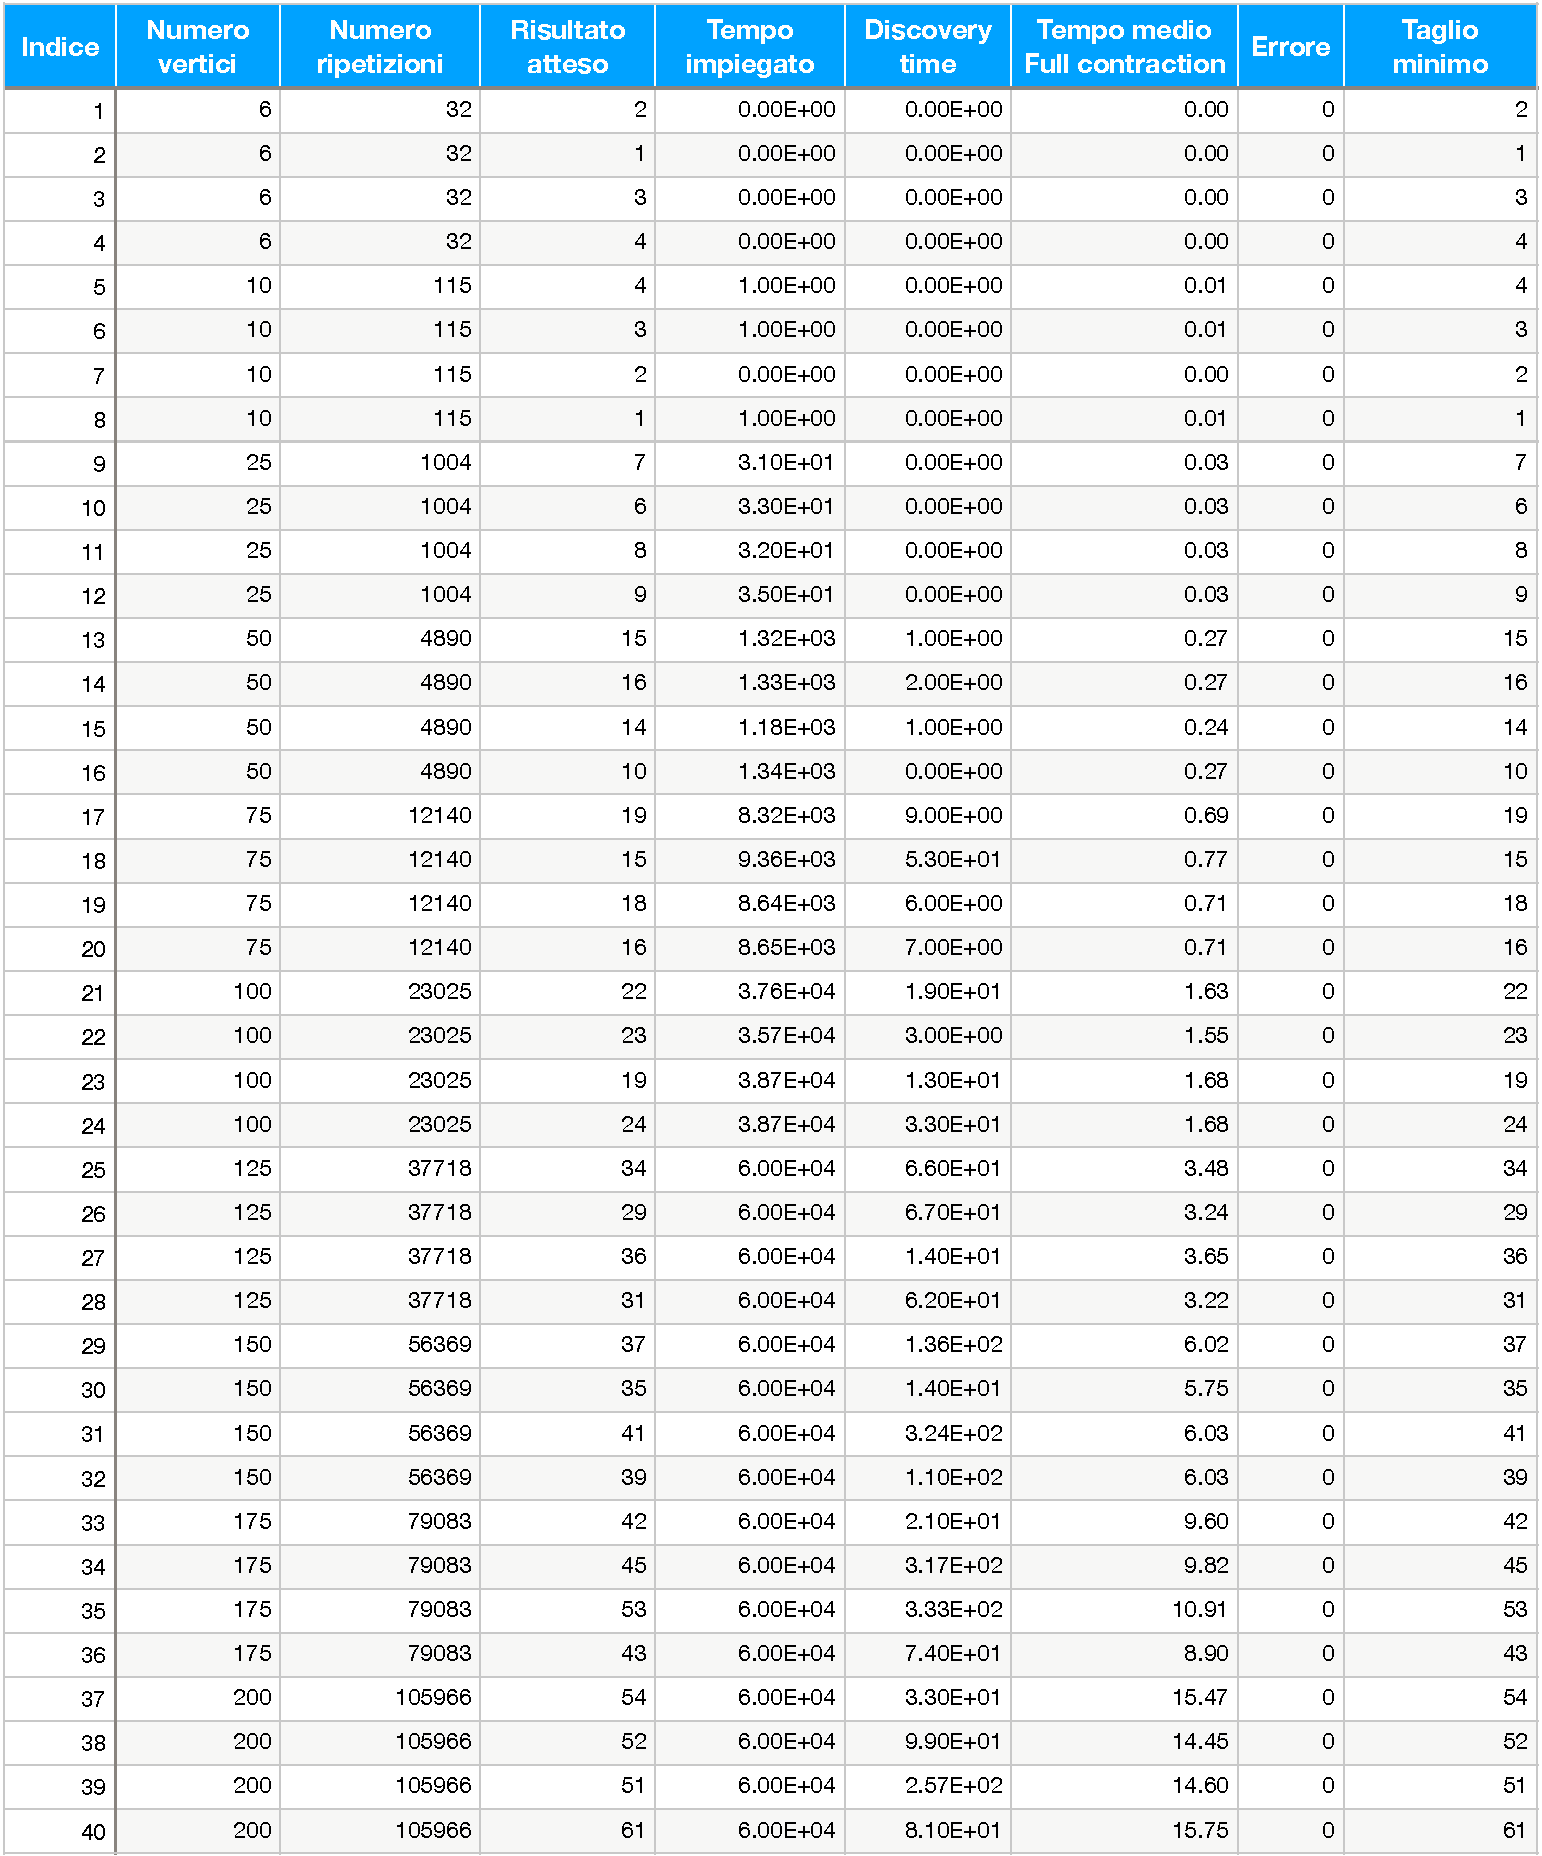
\includegraphics[width=17cm]{tabellapdf}
	\label{fig:tabellapdf}
\end{figure}

\section{Domanda 1}
\begin{figure}[H]
	\centering
	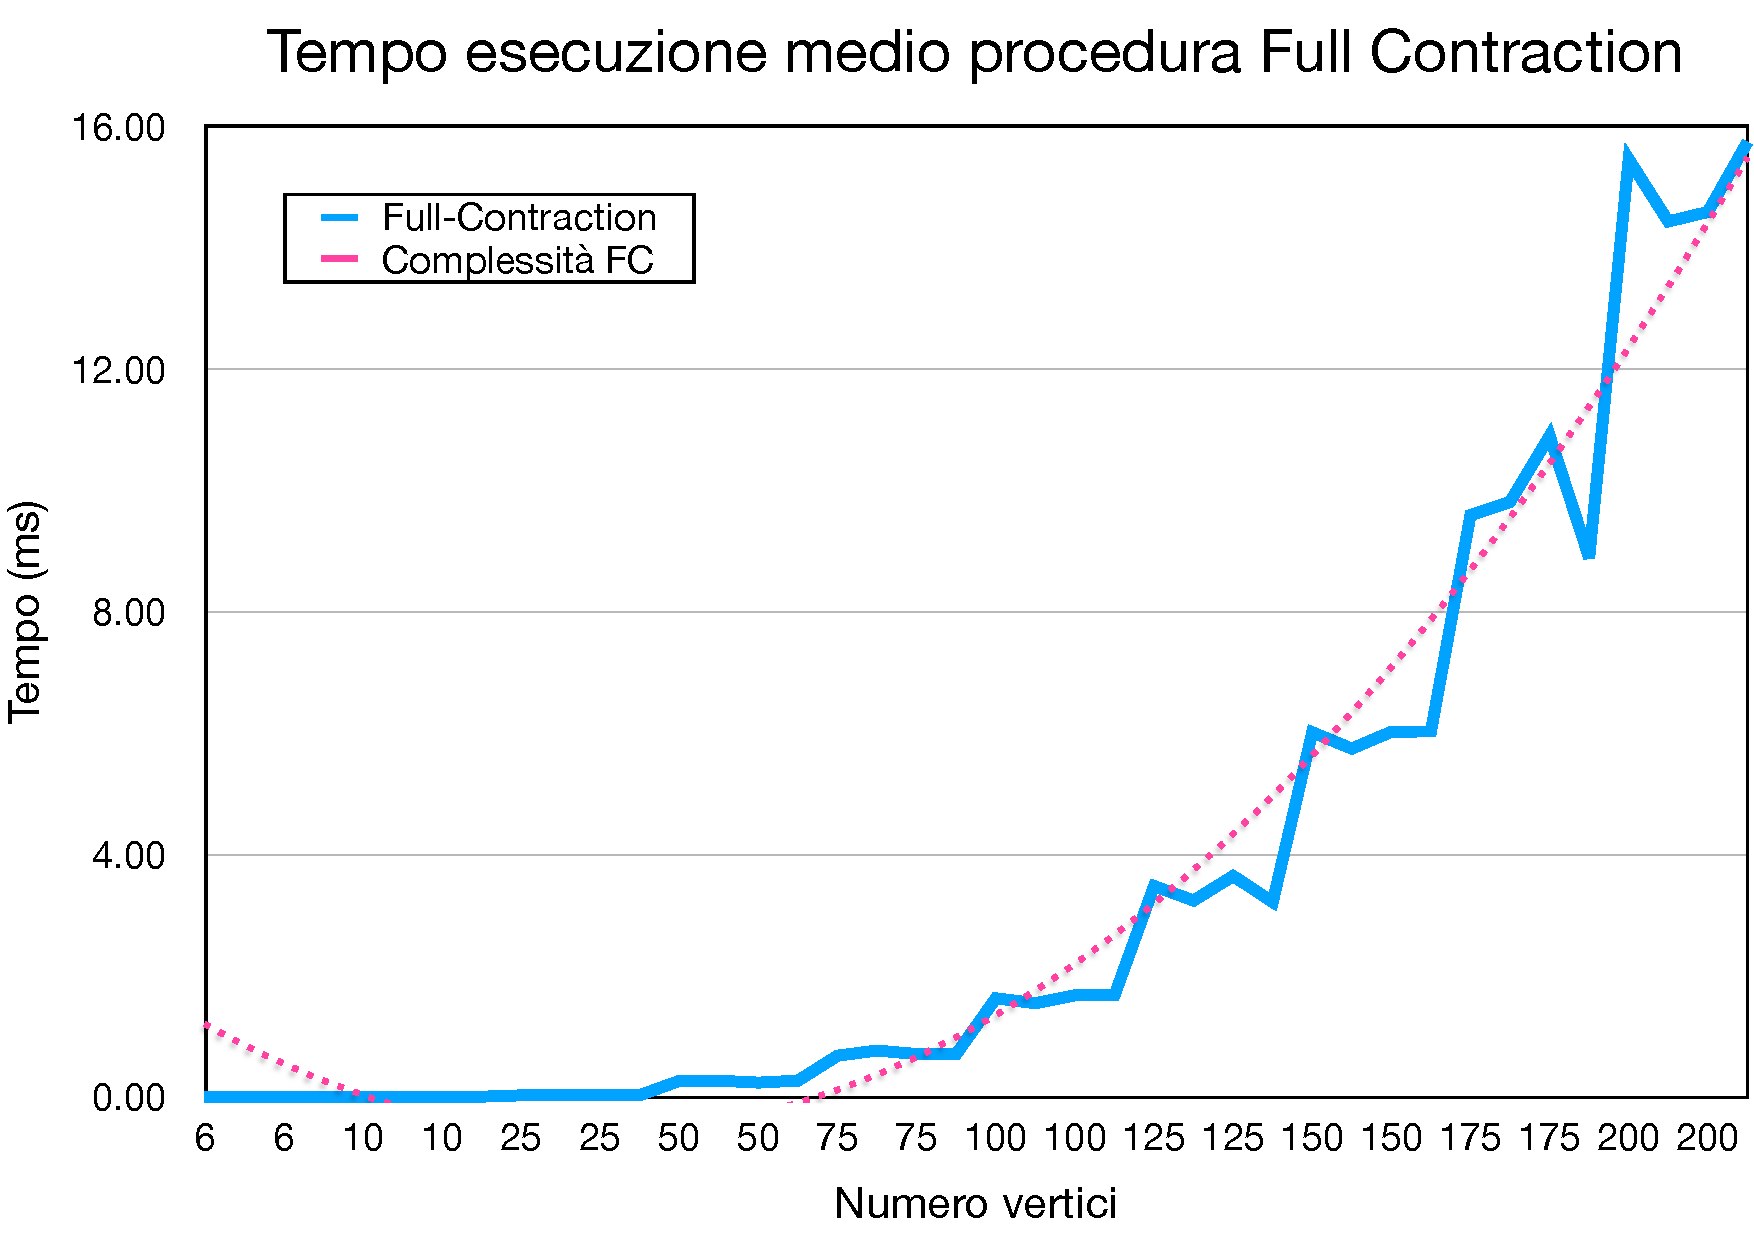
\includegraphics[width=17cm]{fullcontraction}
	\label{fig:fullcontraction}
\end{figure}
Il tempo medio per eseguire una Full-Contraction in base al numero di vertici rimane abbastanza vicino alla sua complessità asintotica

\section{Domanda 2}
\begin{figure}[H]
	\centering
	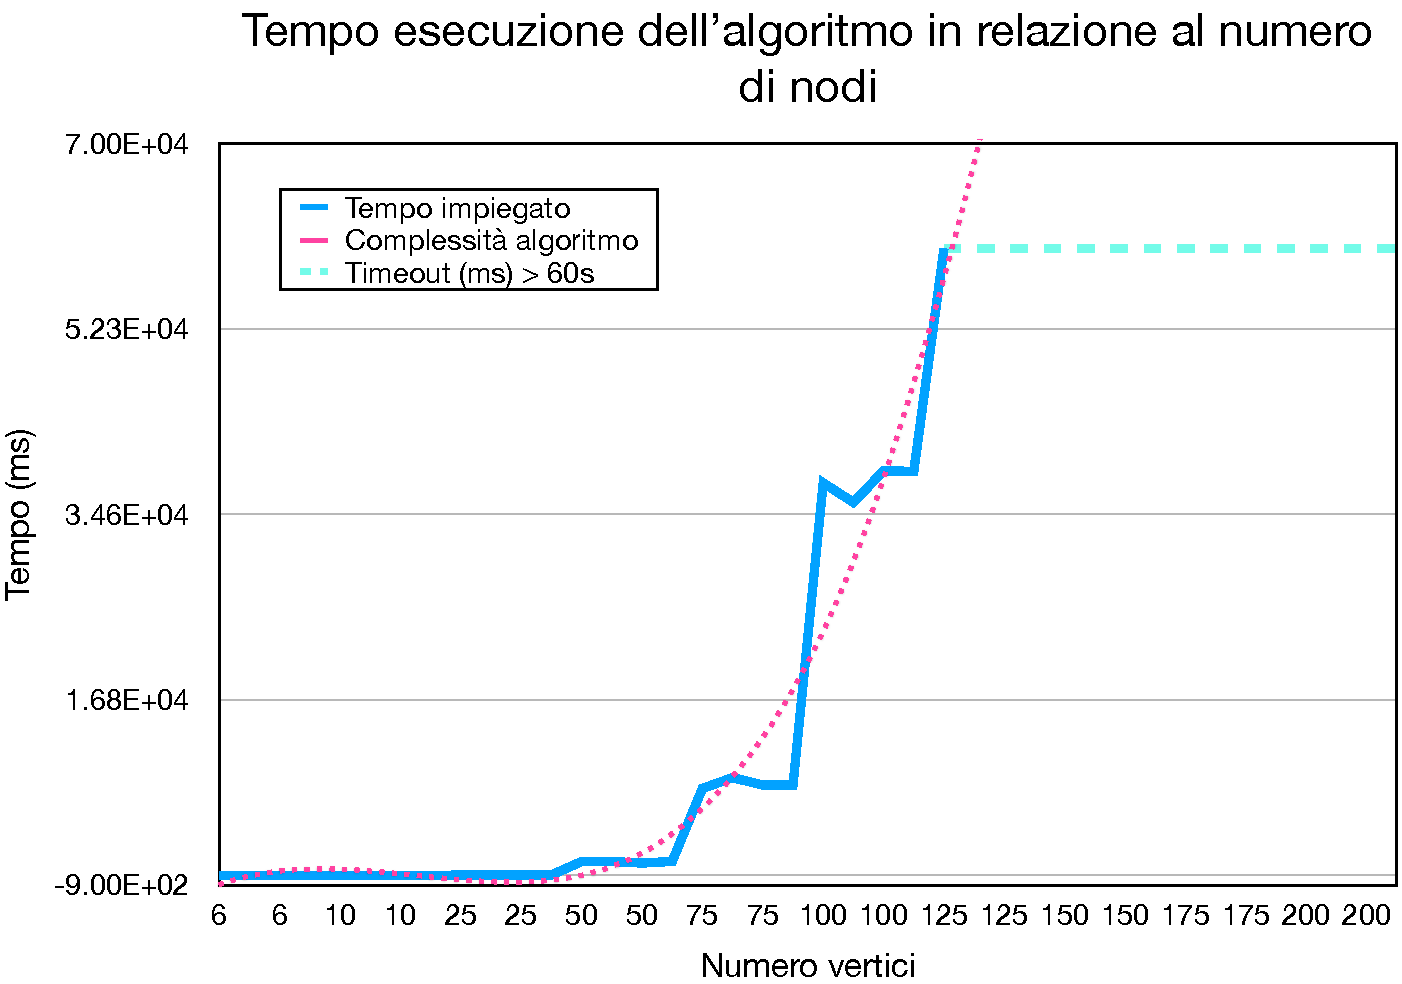
\includegraphics[width=17cm]{tempoesecvsnumnodi}
	\label{fig:tempoesecvsnumnodi}
\end{figure}
Il numero di ripetizioni scelto è $k = (n^2)/2 * log(n)$ dove $n$ è il numero di vertici, in modo da garantire che la probabilità di sbagliare sia minore o uguale a $1/n$.
Il tempo di esecuzione dell'algoritmo segue l'andamento della sua complessità asintotica, ma per i grafi più grandi è stato necessario introdurre un timeout di 60 secondi per mantenere un tempo di esecuzione totale ragionevole.

\section{Domanda 3}
\begin{figure}[H]
	\begin{center}
	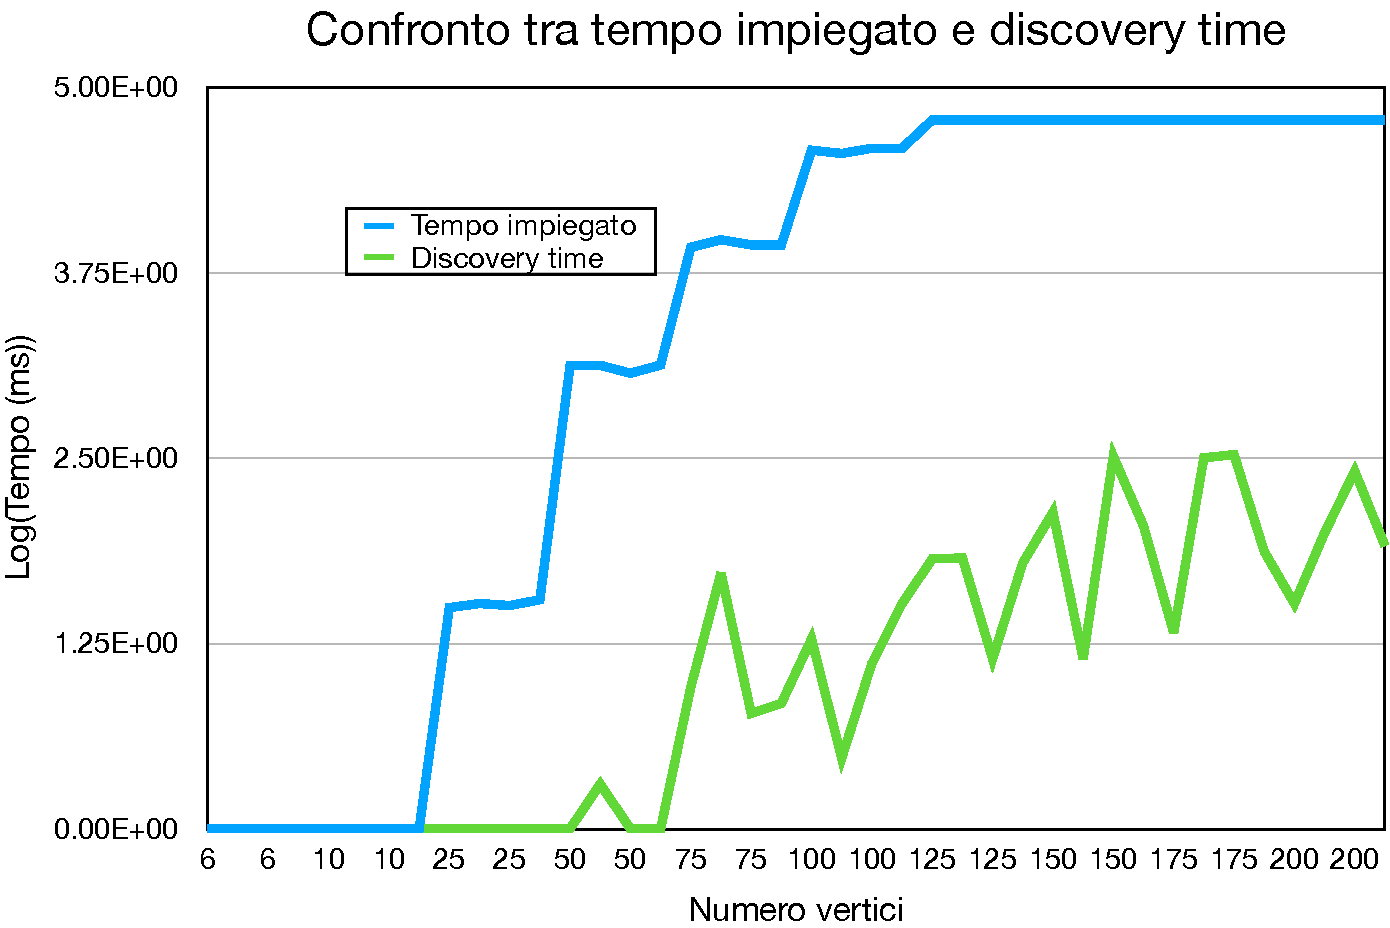
\includegraphics[width=17cm]{discoveryvsfulltime}
	\label{fig:discoveryvsfulltime}
\end{center}
\end{figure}

\section{Domanda 4}
Come si può vedere nella tabella dei risultati nella sezione 2 il taglio ottenuto dall'algoritmo è esattamente il taglio minimo atteso. Questo perché, anche nelle istanze più grandi del dataset, l'algoritmo ha trovato la soluzione ottima prima del timeout di 60 secondi che abbiamo imposto. L'errore relativo è quindi 0 per ogni grafo.

\section{Conclusioni}
L'algoritmo risulta molto efficace a risolvere il problema del minimum cut nonostante la sua semplicità. È interessante notare che il discovery time in genere è molto più breve del tempo di esecuzione totale, e che le iterazioni aggiuntive servono semplicemente a garantire che il risultato sia giusto con alta probabilità. Infatti anche le istanze da 200 vertici hanno ritornato il minimum cut nonostante siano state interrotte molto prima che l'algoritmo completasse tutte le iterazioni. Ovviamente imporre un timeout troppo piccolo riduce drasticamente la probabilità di successo, al punto di rendere l'algoritmo inaffidabile e poco utile per i grafi più grandi.

\end{document}
